\documentclass[a4paper]{article}
\usepackage{lipsum}
\usepackage{url}
\usepackage{graphicx}
\usepackage{listings}
\lstset{language=Python}
\usepackage[margin=2cm]{geometry}
\usepackage{indentfirst}
\usepackage{xcolor}
\usepackage{lmodern}
\usepackage{enumitem}
\renewcommand{\familydefault}{\sfdefault}
\graphicspath{ {images/} }

\begin{document}

% TODO: Anything else needed for titlepage
\begin{titlepage}
	\newcommand{\HRule}{\rule{\linewidth}{0.5mm}}
	\center{}

    %Headings
	\LARGE{University of Nottingham}\\[1.5cm]
	\Large{Computer Science with Artificial Intelligence MSci}\\[0.5cm]
	\large{G54IRP/COMP4027 - Individual Research Project}\\[0.5cm]

    %Title
	\HRule{}\\[0.4cm]
	{\huge\bfseries AI for General Video Game Playing}\\[0.4cm]
	\HRule{}\\[1.5cm]

    %Authors
	\begin{minipage}{0.4\textwidth}
		\begin{flushleft}
			\large
			\textit{Author}\\
			Benjamin Charlton\\
            psybc3@nottingham.ac.uk\\
            4262648
		\end{flushleft}
	\end{minipage}
    \begin{minipage}{0.4\textwidth}
		\begin{flushright}
			\large
			\textit{Supervisor}\\
			Dr.\@ Ender \"Ozcan\\
            Ender.Ozcan@nottingham.ac.uk
		\end{flushright}
	\end{minipage}

    %Date
	\vfill\vfill\vfill
	{\large7\textsuperscript{th} December 2017}
	\vfill

\end{titlepage}

%Contents Page
\pagenumbering{roman}
\tableofcontents
\pagebreak

\pagenumbering{arabic}
\section{Introduction}
\subsection{Introduction}
\begin{itemize}
    \item Popularity of Video Games
    \item Variety of Video games being played
    \item Video Games as a testing ground for AI
\end{itemize}
\subsection{Planning VS learning}
\begin{itemize}
    \item As the title says, just to get some definitions out of the way
\end{itemize}
\subsection{Motivation}
\begin{itemize}
    \item Individual desire to get better at deep reinforcement learning
    \item Learning more Methods
    \item Applying Methods
    \item Learning to use more robust and real world frameworks for DRL \\
    \item Seeing the state of the art in DRL and AI game playing
\end{itemize}
\subsection{Aims and Objectives}
\begin{itemize}
    \item Look at the project plan aims and objectives
\end{itemize}

\section{Related Work}
\subsection{AI and Game Playing}
\begin{itemize}
    \item AI approaches have specialised heuristics or only been developed for a single game
    \\
    \item Early AI and Game playing
    \item Go - previous interim report / PP
    \item Chess - previous interim report / PP
    \item OpenAIFive
    \item GET MORE THINGS FROM PP
    \\
    \item Dartmouth Workshop
\end{itemize}

\subsection{GVGAI and VGDL}
\begin{itemize}
    \item TODO Make some notes up here
\end{itemize}
\subsection{OPEN AI GYM and GVGAI GYM}
\begin{itemize}
    \item What is OPEN AI GYM
    \item Why is OPEN AI GYM helpful for RL
    \item GVGAI GYM
    \item Initial results from GVG AI GYM paper
    \item Maybe some more here :)
\end{itemize}
\cite{GVGAIGYM}
\subsection{Subsection to end all subsections}
\begin{itemize}
    \item Maybe something about the open AI baselines
    \item Depends what technique I would be using but I should look into that
    \item Where does reinforcement learning come into this bad buoy
\end{itemize}


\pagebreak
\section{Appendix}

\subsection{Meeting Minutes}


\pagebreak
\subsection{Work Plan}
% \begin{center}
    % 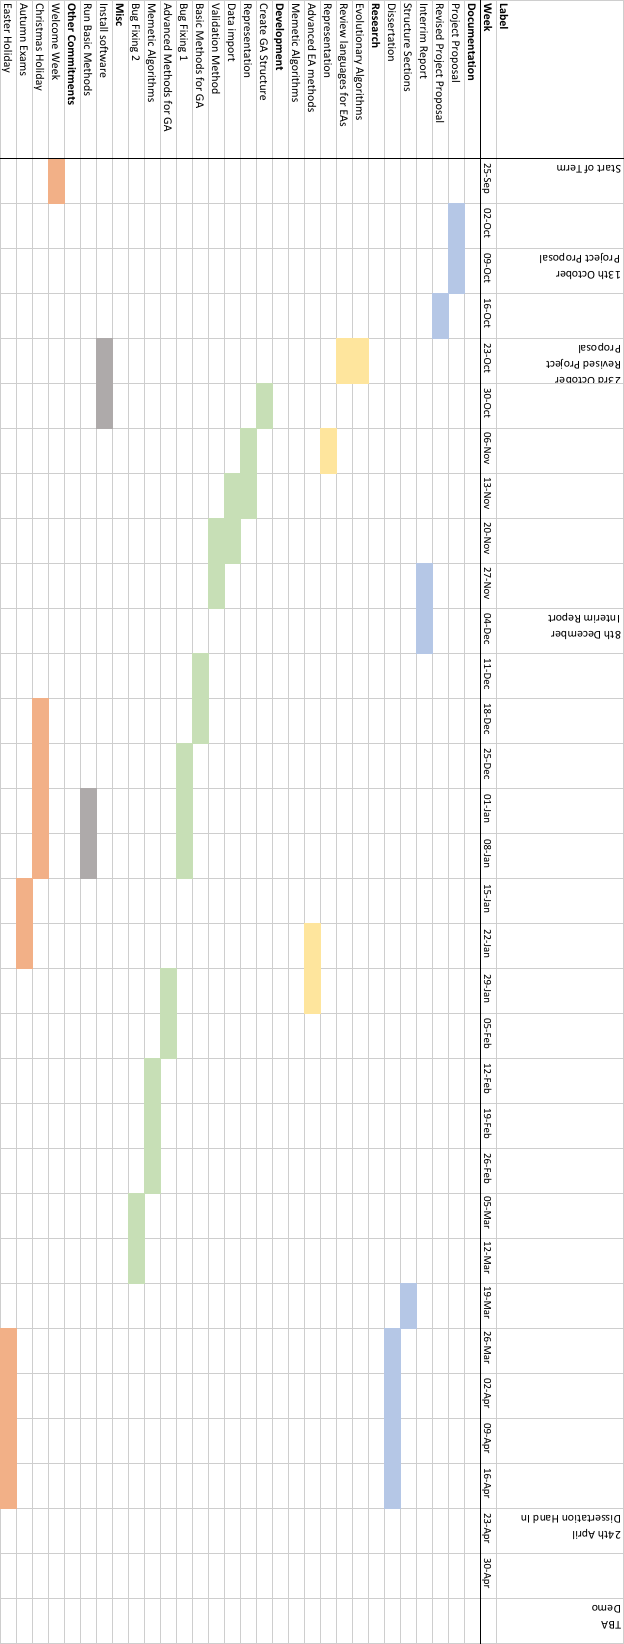
\includegraphics[height=24.8cm]{workPlan.png}
% \end{center}


%Bibliography
\subsection{References}
\bibliography{InterimReport}
\bibliographystyle{plain}


\end{document}
